\documentclass[12pt,a4paper]{book}
\usepackage[utf8]{inputenc}
\usepackage{titlesec}
\usepackage{geometry}
\usepackage{lipsum}
\usepackage{hyperref}
\usepackage{xcolor}
\usepackage[most,breakable]{tcolorbox}
\usepackage{setspace}
\usepackage{fancyhdr}
\usepackage{tikz}
\usetikzlibrary{arrows.meta,positioning}

\geometry{margin=1in}
\setstretch{1.25}

\definecolor{myblue}{RGB}{30,90,150}
\definecolor{mygray}{RGB}{240,240,240}

\hypersetup{
  colorlinks=true,
  linkcolor=myblue,
  urlcolor=myblue
}

\titleformat{\chapter}[display]
  {\normalfont\bfseries\Huge\color{myblue}}
  {\filleft\Large\chaptertitlename\ \thechapter}
  {2ex}
  {\titlerule\vspace{2ex}\filright}
  [\vspace{2ex}\titlerule]

\titleformat{\section}
  {\Large\bfseries\color{myblue}}
  {\thesection}{1em}{}

\pagestyle{fancy}
\fancyhf{}
\fancyhead[L]{\leftmark}
\fancyhead[R]{\thepage}

\newtcolorbox{notebox}[1][]{
  colback=mygray,
  colframe=myblue,
  fonttitle=\bfseries,
  title=#1,
  sharp corners,
  boxrule=1pt,
  breakable
}

\title{Note of \textit{Principles of Communications}}
\author{Zhehao Yi}
\date{Sep 18. 2025}

\begin{document}

\maketitle
\tableofcontents
\newpage

\chapter{Chapter 1: Introduction}
When one consider the technological developments that make such instantaneous information access possible, two main ingredients surface - a reliable, fast means of communication and a menas of storing the information for ready access, sometimes referred to as the \textit{convergence} of communications and computing.

A system is a combination of circuits and/or devices that is asssemvled to caccomplish a desired task.

A characteristic of electrical communication systems is \textit{the presence of uncertainty}. This uncertainty is due in part to inevitable presence in any system of unwanted signal perturbations, broadly referred to as \textit{noise}, and in part to the unpredictable nature of information itself.

System analysis in the presence of such uncertainty requiresthe use of probabilistic techniques.

Why the alomost complete domination by digital formatting in today's world?
\begin{itemize}
  \item Media integrity - a dgital format sufffers much less deterioration in reproduction than does an analog record.
  \item Media integration - whether a sound, picture, or naturallt digital data such as a word file, all are treadted the same when in digital format.
  \item Flexible interaction - the digital domain is much more convenient for supporting anything from one-on-one to many-to-many interactions.
  \item Editing - whether text, sound, image, or video, all are conveniently and easily edited when in digital format. (Is this the reason why we need protect our information from been edited?)
\end{itemize}
\section{The Block diagram of a Communication System}
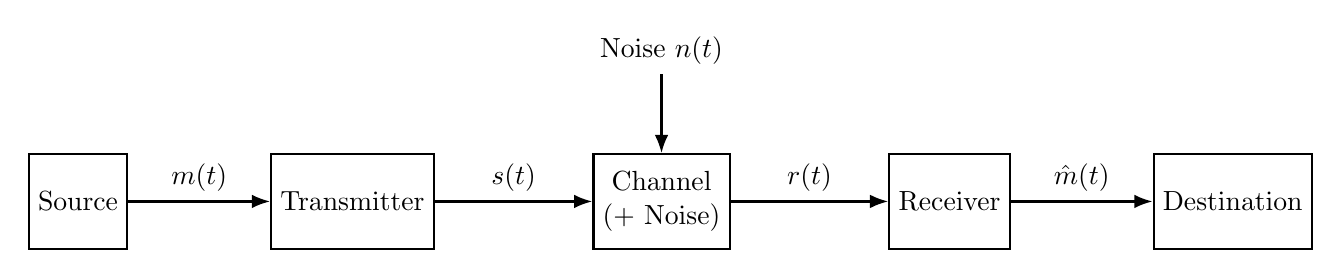
\begin{tikzpicture}[
  block/.style={draw, thick, minimum width=1.0cm, minimum height=1.2cm, align=center},
  >={Latex}
]

% Nodes
\node[block] (src) {Source};
\node[block, right=1.8cm of src] (tx) {Transmitter};
\node[block, right=2.0cm of tx] (ch) {Channel\\(+ Noise)};
\node[block, right=2.0cm of ch] (rx) {Receiver};
\node[block, right=1.8cm of rx] (dst) {Destination};

% Connections
\draw[->, thick] (src) -- (tx) node[midway, above] {$m(t)$};
\draw[->, thick] (tx) -- (ch) node[midway, above] {$s(t)$};
\draw[->, thick] (ch) -- (rx) node[midway, above] {$r(t)$};
\draw[->, thick] (rx) -- (dst) node[midway, above] {$\hat{m}(t)$};

% Noise arrow into channel
\node[above=1.0cm of ch] (n) {Noise $n(t)$};
\draw[->, thick] (n) -- (ch);

\end{tikzpicture}
Above shows a commonly used model for a single-link communication system. This block diagram is also applicable to remote sensing system, such as radar or sonar, in which the system input and output may be located at the same site.

Before the Transmitter, we usually have a input transducer.

\textbf{\textit{Input Transmitter}}: Convert the message produced by a source to a form suitable for the particular type of communication system.

\textbf{\textit{Transmitter}}: The purpose of the transmitter is to couple the message to the channel. In some intercom systems, it is often necessary to \textit{modulate} a carrier wave with the signal from the input transducer. \textit{Modulation} is the systematic variation of some attribute of the carrier, such as amplitude, phase, or frequency, in accordance with a function of the message signal. There are several reasons for using a carrier and modulating it.
\begin{itemize}
  \item For ease of radiation.
  \item To reduce noise and interference.
  \item For channel assignment.
  \item For multiplexing or transmission of several messages over a single channel.
  \item To overcome equipment limitations.
\end{itemize}
in addition the modulation. other primary functions performed bt the transmitter are filtering, amplification, and coupling the modulated signal to the channel.

\textbf{\textit{Channel}}: The signal undergoes degradation from transmitter to receiver.

\textbf{\textit{Receiver}}: The receiver's function is to extract the desired message from the received signal at the channel output and to convert it to a form suitable for the output transducer.

\textbf{\textit{Output Transducer}}: This output transducer completes the communication system. This devices converts the electric signal at its input into the form desired by the system user.
\section{Channel Characteristics}
\subsection{Noise Source}
Depends on the noise source, noise in communication system can be classified into two broad categories.
\begin{itemize}
  \item Noise generated by components within a communication system, such as resistors and solid-state active devices is reffed to as \textit{internal noise}.
  \item Noise comes from outside of communication system called \textit{external noise}, including atmospheric, man-made, and extraterrestrial sources.
\end{itemize}

Atmospheric noise results primarily from spurious radio waves (by the natural electrical discharges, within the atmosphere associated with thunderstorms). It is commonly referred to as \textit{static} or \textit{spherics}. Atmospheric noise is characterized in the time domain by large-amplitude, short duration bursts and is one of the prime examples of noise referred to as \textit{impulsive}. Because of its inverse dependence on frequency, atmospheric noise affects commercial AM broadcast radio, which occupies the frequency range from 540kHZ to 1.6MHZ, more than it affects television and FM radio, which operate in frequency bands above 50MHZ.

Man-made nosie sources include 
high-voltage powerline corona discharge, 
commutator-generated noise in electrical motors,
automobile and aircraft ignition noise, and switching-gear noise. impulsive noise is the predominant type of noise in switched wireline channels, such as telephone channels (can be a serious source or error in applications involving transmission of digital data).

Noise due to interfering transmitters is commonly referred to as \textit{radio-frequency interference}(RFI)
RDI is particularly troublesome in situations in which a receiving antenna is subject to a high-density transmitter environment,
as in mobile communications in a large city.

If the scattering mechanism results in numerous reflected components, the received multipath signal is noiselike and is termed \textit{diffuse}

If the multipath signal component is composed of only one or two strong reflected rays, it is termed \textit{specular}

Such signal perturbations are referred to as \textit{fading}

Internal noise results fro the random motion of charge carriers in electronic components, can be of three general types: the first is referred to as \textit{thermal noise} (random motions of free electrons in a conductor or semiconductor excited by thermal agitation), the second is called \textit{short noise} (random arrival of discrete charge carriers in such devices as thermionic tubes or semiconductor junction devices), the third is called \textit{flicker noise} (is produced in semiconductors by a mechanism not well understood and is more sever the lower frequency).

\subsection{Types of Transmission channels}
Discuses the characteristics, advantages, and disadvantages of three common types: electromagnetic-wave propagation channels, guided electromagnetic-wave channels, and optical channels.
The characteristics of all three may be explained on the basis of electromagnetic-wave propagation phenomena.

\textbf{Electromagnetic-Wave Propagation Channels}

The basic physical principle involved is the coupling of electromagnetic energy into a propagation medium,
which can be free space or the atmosphere, by means of a radiation element referred to as an \textit{antenna}.

The VHF (Vary High Frequency) band has 10 times as much frequency space as the HF band.

At lower frequencies, or long wavelengths, propagating radio waves tend to follow the earth's face. At higher frequencies, or short wavelengths, radio waves propagate in straight line.
Another phenomenon that occurs at lower frequencies is reflection of radio waves by the ionosphere.

WiMax (Worldwide Interoperability for Microwave Access) sometimes referred to as Wi-Fi on steroids.
The differences between Wi-Fi and WiMax are listed below:
\begin{itemize}
  \item Wi-Fi is LAN (Local Area Network), WiMax is WAN (Wide Area Network).
  \item Wi-Fi operates in unlicensed spectrum, WiMax operates in licensed spectrum.
\end{itemize}

\textbf{Guided Electromagnetic-Wave Channels}

By 1952, use of the types of modulation known as double-sideband and single-sideband on high-frequency carriers was established. Communication over predominantly multipair and coaxial-cable lines produced transmission of much better quality.

However, with the development of low-loss optical fibers, efforts to improve millimeter-wave systems to achieve greater bandwidth ceased.

\textbf{optical Links}

The technological breakthroughs that proceeded the widespread use of light waves for communication were the development of small coherent light sources (semiconductor lasers), low-loss optical fibers or waveguides, and low-noise detector.

\section{Summary of System-Analysis Techniques}
\subsection{Time and Frequency-domain Analyses}

\subsection{Modulation and Communication Theories}

\section{Probabilistic Approaches to System Optimization}
\begin{notebox}[Summary]
some summary
\end{notebox}

\section{Summary}
\begin{notebox}[Thinking]
some thinking
\end{notebox}

\chapter{Chapter 2:}
\section{}
\begin{notebox}[Summary]
some summary
\end{notebox}

\section{}
\begin{notebox}[Concept]
some concept 
\end{notebox}

\section{}
\begin{notebox}[Thinking]
some thinking
\end{notebox}

\end{document}
